% !TEX TS-program = xelatex

% Inicializace tulthesis
\documentclass[FM]{tulthesis}
% Typografie pro češtinu; xelatex alternativa pro babel
\usepackage{polyglossia}
\setdefaultlanguage{czech}
% Automatické pevné mezery
\usepackage{xevlna}

% Pro seznam použité literatury
\usepackage[backend=biber, style=iso-numeric]{biblatex}
\addbibresource{zdroje.bib}

% Titulní strana
\TULtitle{Tvorba a využití botu pro výuku matematiky na platformě Discord}{Creating and using a bot for teaching mathematics on the Discord platform}
\TULprogramme{B0613A140005}{Informační technologie}{Information technology}
%\TULbranch{B0613A140005AI}{Aplikovaná informatika}{Applied Informatics}
\TULauthor{Radek Mocek}
\TULsupervisor{Ing.  Igor Kopetschke}
\TULyear{2024}

% Začátek dokumentu
\begin{document}
	% Prohlášení
	\ThesisStart{male}
	
	% Poděkování
	\begin{acknowledgement}
		Děkuji
	\end{acknowledgement}
	
	% Abstrakt česky
	\begin{abstractCZ}
		Abstrakt česky
	\end{abstractCZ}
	
	% Klíčová slova česky
	\begin{keywordsCZ}
		Klíčová slova česky
	\end{keywordsCZ}
	\vspace{2cm}
	
	% Abstrakt anglicky
	\begin{abstractEN}
		Abstrakt anglicky
	\end{abstractEN}
	
	% Klíčová slova anglicky
	\begin{keywordsEN}
		Klíčová slova anglicky
	\end{keywordsEN}
	
	% Obsah
	\tableofcontents
	
	% Seznam obrázků
	\listoffigures
	
	% Seznam tabulek
	%\listoftables
	
	\clearpage
	
	% Zkratky
	\begin{abbrList}
		\textbf{API} & application programming interface \\
		\textbf{SDK} & software development kit \\
		\textbf{VoIP} & Voice over Internet Protocol \\
		\textbf{UI} & user interface \\
	\end{abbrList}
	
	% Začátek hlavního textu
	
	% 1. Vypracujte rešerši sociálních platforem, které umožňují integraci botů.
	% 2. Analyzujte vybranou skupinu existujících botů na platformě Discord a knihoven pro jejich tvorbu.
	% 3. Navrhněte bot zaměřený na výklad a příklady z lineární algebry při využití specifických funkcí Discordu včetně administrace a interaktivních zpráv.
	% 4. Navržené řešení implementujte a nasaďte do testovacího provozu pro vybranou skupinu uživatelů.
	% 5. Vyhodnoďte zpětnou vazbu od uživatelů a navrhněte případné úpravy a vylepšení.
	
	\chapter{Úvod}
	
	Úvod.
	
	\chapter{Boti na sociálních platformách}
	
	Tato kapitola představuje Discord a některé další sociální platformy, které přímo podporují tvorbu a integraci botů. Nejdříve je ale nutné upřesnit, jak jsou v tomto kontextu myšleny výrazy \textit{sociální platforma} a \textit{bot}.
	
	Discord je vcelku obtížné zařadit do jedné konkrétní kategorie softwaru. Dokud se nově zaregistrovaný uživatel nepřipojí na žádný server, pak se Discord chová jako VoIP a instant messaging aplikace, kde lze komunikovat pouze s lidmi, které si uživatel přidá do přátel. Po připojení na nějaký veřejný Discord server se ale aplikace přibližuje ke kategorii sociálních médií, kdy uživatel může sdílet a konzumovat obsah v rámci moderované komunity. Pojem sociální platforma je zde tedy myšlen spíše jako zastřešující termín pro Discord a jemu podobné aplikace, u nichž o zařazení do této kapitoly především rozhodovalo, zdali nějakým způsobem podporují integraci botů.
	
	Uživatelé sociálních médií často vnímají pojem bot negativně, jelikož se mezi boty mimo jiné řadí i programy generující spam nebo umělou návštěvnost za účelem zkreslení statistik \cite{lit3}. Na platformách zkoumaných v této kapitole je ale bot speciální typ uživatele, jehož chování je automatizované a určené programem. Tento bot je obvykle přidán do skupinové konverzace, kde pak za pomoci volání API dané platformy dokáže provádět stejné akce jako běžný uživatel. Jedná se například o odesílání zpráv a čtení jejich obsahu, moderaci členů serveru, nebo i připojení do hlasového hovoru. Nemusí se jednat o chatbota, který se snaží imitovat lidské chování. Bot obvykle reaguje na předem danou sadu příkazů vykonáním nějaké činnosti.
	% Historie, pricing, open/closed source, kompatibilita, FEATURES, BOTI
	\section{Discord}
	
	Platforma Discord vznikla v roce 2015 jako reakce na nedostatky tehdejších služeb pro online komunikaci mezi hráči videoher \cite{lit3}. S nabývající popularitou se ale na Discordu začaly objevovat veřejné komunity zaměřené nejen na téma videoher. Často se jedná o oficiálně vytvořené servery náležící k nějakému produktu, které slouží jako diskuzní fórum a propagace zároveň. Momentálně je například největší komunitou (podle počtu členů) server Midjourney, který patří ke stejnojmennému nástroji pro tvorbu obrázků pomocí umělé inteligence. Uživatelé zde mohou o nástroji diskutovat, hlásit chyby, sdílet vytvořené obrázky, nebo je nechat generovat pomocí Midjourney bota.
	
	Discord lze používat ve webovém prohlížeči, nebo jsou k dispozici aplikace pro počítače a mobilní zařízení. Základní verze je zdarma s možností měsíčního předplatného \textit{Discord Nitro}. Předplatitelé mají navíc k dispozici kosmetické prvky (např. vlastní emotikony nebo animovaný avatar) a některé základní funkce jsou pro ně vylepšeny (např. nahrávání větších souborů nebo streamování videa ve vyšším rozlišení). Licence je proprietární.
	
	% DMs, voice, group;; Servery – kanály, role, threads, události, nastavení komunity (announcements, discussions)
	Program disponuje obvyklou instant messaging a VoIP funkcionalitou. V tzv. přímých zprávách si mezi sebou uživatelé mohou posílat textové zprávy a soubory. Dále je k dispozici hlasová komunikace s případným sdílením obrazovky nebo videa z webkamery. Tyto akce lze provádět i v soukromých skupinách, které ale mají omezený počet deseti uživatelů.
	% Boti – co dokážou (API) (i omezení, historie, bot vs aplikace, ...), obvyklé kategorie
	
	\section{Slack}
	
	Z populárních a hojně používaných platforem se Discordu vzhledově i funkčně nejvíce podobá program Slack. Ten byl spuštěn již v roce 2013 a od té doby si vybudoval reputaci jako standard pro komunikaci v technologických společnostech. \cite{lit3}
	
	Slack se prezentuje jako software usnadňující interní komunikaci v nějaké organizaci a dal by se nazvat jako \quotedblbase Discord pro firmy\textquotedblleft\,. Tomu odpovídá i zdejší výběr tzv. aplikací (\textit{Apps}), které se podobají zkoumaným botům. Tyto aplikace se zaměřují především na zvýšení produktivity, teambuilding, nebo integraci již existující služby třetí strany do prostředí Slacku.
	
	\begin{figure}[ht]
		\centering
		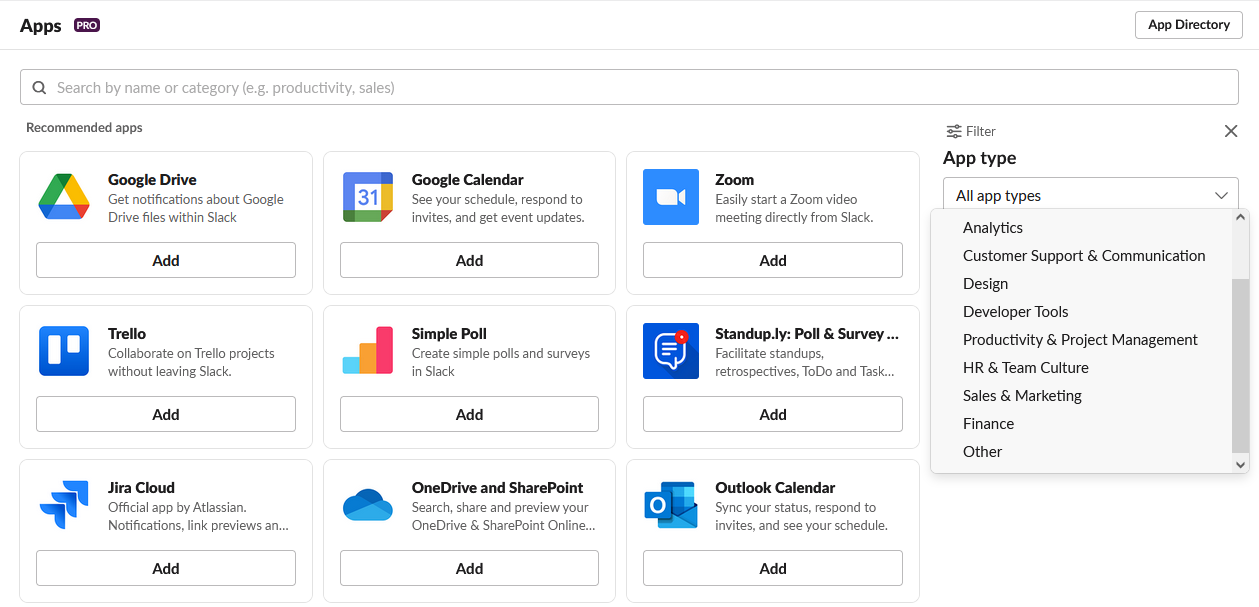
\includegraphics[width=\textwidth]{img/SlackApps}
		\caption{Doporučené Slack aplikace}
	\end{figure}
	
	Stejně jako uživatelé mohou Slack aplikace spravovat konverzace a odesílat do nich textové zprávy. % TODO https://api.slack.com/start/apps
	
	Zorientovat se v procesu tvorby Slack aplikací nemusí být jednoduché. Tyto aplikace se totiž dělí na klasické (\textit{classic}) a nové (zvané \textit{modern} nebo \textit{next-generation}, představené v roce 2021), jejichž API se liší. Ani slovo bot není ve Slack ekosystému jednoznačné. U klasických aplikací se jedná o jejich speciální typ, se kterým je komunikace vedena běžnou řečí namísto příkazů nebo UI (chatbot). Tento bot je označen jako \textit{legacy} a v budoucnu pravděpodobně nebude podporován. U nového typu aplikací se z pohledu uživatele slovo bot nikde nevyskytuje (maximálně v názvu nějaké aplikace), z dokumentace je ale zjevné, že se (stejně jako u Discordu) jedná o speciálního uživatele ovládaného danou aplikací, tato informace však není nikde explicitně zmíněna. Při práci s dokumentací nebo neoficiálními návody je tedy nutné dávat pozor na to, s jakou technologií daný manuál pracuje, protože může dojít ke snadné záměně výše zmíněných pojmů.
	
	Klasické Slack aplikace lze vyvíjet v řadě komunitních knihoven a musí být hostovány na vlastním serveru. \textit{Next-generation apps} pak mají připravené oficiální SDK a o hosting se stará přímo Slack, pro jejich vývoj a následné nasazení je ale nutné mít Slack ve placené verzi.
	
	% https://revolt.chat/
	% https://matrix.org/
	% https://www.guilded.gg/
	% Teams
	% flock
	% rocket.chat
	% FB Messenger
	
	\chapter{Matematika na platformě Discord}	
		
	\chapter{Tvorba Discord bota}
	
	\section{Prostředky pro tvorbu}
	
	\section{Návrh}
	
	\section{Implementace}
	
	\section{Zhodnocení}
	
	\chapter{Závěr}
	
	Závěr.
	
	% Zdroje
	\chapter*{Seznam použité literatury}
	\addcontentsline{toc}{chapter}{Seznam použité literatury}
	\printbibliography[heading=none]
	
\end{document}